\documentclass{article}

\usepackage{geometry}
\usepackage{makecell}
\usepackage{array}
\usepackage{multicol}
\usepackage{setspace}
\usepackage{multicol}
\usepackage{changepage}
\usepackage{wrapfig}
\usepackage[ngerman]{babel}
\usepackage{booktabs}
\usepackage{csquotes}
\usepackage{lipsum}
\usepackage[explicit]{titlesec}
\usepackage{graphicx}
\usepackage{cprotect}
\usepackage{float}
\usepackage{hyperref}
\newcolumntype{?}{!{\vrule width 1pt}}
\newcommand\HREF[2]{\hyper@linkurl{#2}{#1}}
\newcommand{\paragraphlb}[1]{\paragraph{#1}\mbox{}\\}
\renewcommand{\contentsname}{Inhaltsverzeichnis:}
\renewcommand\theadalign{tl}
\setstretch{1.20}
\setlength{\parindent}{0pt}
\renewcommand{\thesubsection}{\alph{subsection}}
\renewcommand{\thesubsubsection}{\roman{subsubsection}}

\titleformat{\section}
  {\normalfont\Large\bfseries}{\thesection}{1em}{\hyperlink{sec-\thesection}{#1}
\addtocontents{toc}{\protect\hypertarget{sec-\thesection}{}}}
\titleformat{name=\section,numberless}
  {\normalfont\Large\bfseries}{}{0pt}{#1}

\titleformat{\subsection}
  {\normalfont\large\bfseries}{\thesubsection}{1em}{\hyperlink{subsec-\thesubsection}{#1}
\addtocontents{toc}{\protect\hypertarget{subsec-\thesubsection}{}}}
\titleformat{name=\subsection,numberless}
  {\normalfont\large\bfseries}{\thesubsection}{0pt}{#1}

\hypersetup{
    colorlinks,
    citecolor=black,
    filecolor=black,
    linkcolor=black,
    urlcolor=black
}



\geometry{top=12mm, left=1cm, right=2cm}

\begin{document}
	\begin{titlepage}
		\centering
		
\includegraphics[width=0.25\textwidth]{Bilder/02logo.png}\par\vspace{1cm}
		{\scshape\LARGE FH Campus 02 \par}
		\vspace{1cm}
		{\scshape\Large Web Technologien und Usability \\ Gruppenabgabe\par}
		\vspace{1.5cm}
		{\huge\bfseries Heuristische Evaluierung\par}
		\vspace{2cm}
		{\Large\itshape {\LARGE \bfseries B1-Kronehit} \vspace{1cm} \\ Andreas Hofer \\ Hannah Posch \\ Samuel Ulz\par}
		\vfill
		{\large \today\par}
	\end{titlepage}
	\tableofcontents
	\newpage
	\section{Grundinformation}
	Ziel dieser heuristischen Evaluierung war die Websites des Privatradiosenders Kronehit \href{https://kronehit.at}{kronehit.at}. Als Basis für die Analyse wurden die Heuristiken von Keith Andrews verwendet. An dieser Evaluation teilgenommen haben: \textbf{Andreas Hofer}, \textbf{Hannah Posch} und \textbf{Samuel Ulz}. Da es nicht möglich scheint Videos in PDFs einzubetten, wurden diese im Anhang verlinkt und, falls relevant ein Ausschnitt davon als Bild eingebettet.
	\section{Zusammenfassung}
	Dieser Bericht befasst sich mit der heuristischen Evaluation von \href{https://kronehit.at}{kronehit.at}. Aus Sicht des Evaluationsteams war der schwerwiegendste Fehler die nicht-triviale Menge an toten Links innerhalb der Website. In mindestens zwei Fällen führte ein vermeintlicher Link zu einer Ressource welche nicht mehr verfügbar war. Manche Elemente scheinen in iOS-basierten Browsern auch unverändert aus Vorlagen übernommen und bieten so Funktionen an, welche die Website nicht anbietet. Ein weiterer Punkt ist der Radioplayer, welcher nur über den Footer erreichbar ist und an manchen Stellen eine relativ mangelhafte Funktionalität aufweist. \\ \\
	Es gibt jedoch auch positives hervorzuheben. So erwies sich die Funktion des Radioplayers auf der Hauptseite als sehr angenehm. Zusätzlich bietet die Seitenleiste gegenüber dem etwas vollen Design der Hauptseite eine sehr komfortable Methode um alle Hauptfunktionen der Website erreichen zu können. \\ \\
	Im Allgemeinen weist die Website von Kronehit einige grobe Mängel auf, welche oft nicht durch durch fehlerhaftes Design ausgelöst werden sondern mehr von technische Natur sind. Kronehit.at scheint auch an manchen Stellen nur mangelhaft für mobile Browser ausgelegt zu sein, was zu einigen scherwiegenden iOS-spezifischen Problemen führt. Designelemente wie der Radioplayer oder die Seitenleiste sind jedoch durchaus gelungen.
	\section{Website}
	Die Website des Senders hat mehrere große Themengebiete, welche fließend ineinander übergehen. Elemente sind stets in Kacheln angeordnet mit einer Angabe zu welchem der Themengebiete sie gehören:
	\begin{itemize}
		\item{Webradio}
		\begin{itemize}
			\item{Der wichtigste Teil des Auftritts und von allen Unterseiten aufrufbar. Zusätzlich zu den regulären, mittels UKW empfangbaren Sender, bietet die Website auch einige Sender nur auf der Website an}
		\end{itemize}
		\item{Nachrichten}
		\begin{itemize}
			\item{Kronehit.at bietet auch Kurznachrichten in einem eigenen Reiter an}
		\end{itemize}
		\item{Gewinnspiele}
		\begin{itemize}
			\item{Es finden oft Gewinnspiele statt, welche in der Regel von Unternehmen gesponsert werden.}
		\end{itemize}
		\item{Services}
		\begin{itemize}
			\item{Zusätzlich bietet die Website einige Services an:}
			\begin{itemize}
				\item{Wetter - Nur für große Städte und nur pro Tag}
				\item{Verkehr - Verlinkt auf die Website des ÖAMTC}
				\item{Frequenzfinder - Gibt die Frequenz des Senders anhand der Postleitzahl an}
				\item{Hitsuche - Zeigt gespielte Hits zu einer bestimmten Zeit an}
			\end{itemize}
		\end{itemize}
	\end{itemize}
	\section{Evaluierung}
	\subsection{Benutzerprofile}
	Anhand der Funktionen der Website haben wir drei Benutzergruppen erstellt:
	\begin{itemize}
		\item{Buchhalterin}
		\begin{itemize}
			\item{Helga, 40, arbeitet in einem Büro und hört nebenbei auf der Website von kronehit Radio. Sie ist besonders an den Online-only Radios interessiert.}
		\end{itemize}
		\item{Eventgänger}
		\begin{itemize}
			\item{Max, 25, geht gerne auf Konzerte und andere Events und verwendet den Eventkalender der Website um Events in ihrer Nähe zu finden.}
		\end{itemize}
		\item{Kurznachrichten}
		\begin{itemize}
			\item{Franz, 55, verwendet den Onlineauftritt von Kronehit um über die neuesten Nachrichten informiert zu werden.}
		\end{itemize}
	\end{itemize}
	\subsection{Evaluierungsumgebung}
	Um reale Nutzungsbedigungen widerzuspiegeln, wurden Mobile- sowie Desktopbrowser mit und ohne Ad Blocker verwendet. Konkret sahen die Testumgebungen wie folgt aus:
	\begin{center}
		\begin{tabular}{? l | l ?}
			\toprule
			\multicolumn{2}{? c ?}{\textbf{Andreas Hofer (ah)}} \\ \midrule
			Gerät: &  MacBook Pro 2016 \\ \hline
			OS: & MacOS 12.7.6 \\ \hline
			Browser: & Safari 17.6 \\ \hline
			AdBlocker: & Keiner \\ \hline
			Datum: & 28.5.2025 \\ \hline
			Zeit: & 15:30 - 17:00 \\ \hline
			Aufnahme: & MacOS Screen Recorder \\
			\bottomrule
		\end{tabular}
		\begin{tabular}{? l | l ?}
			\toprule
			\multicolumn{2}{? c ?}{\textbf{Hannah Posch (PH)}} \\ \midrule
			Gerät: & Lenovo Thinkpad \\ \hline
			OS: & Windows 11 \\ \hline
			Browser: & Mozilla Firefox 139.0.4 \\ \hline
			AdBlocker: & Ghostery \\ \hline
			Datum: & 26.5.2025 \\ \hline
			Zeit: & 18:00 - 19:30 \\ \hline
			Aufnahme: & OBS Studio \\
			\bottomrule
		\end{tabular}
		\begin{tabular}{? l | l ?}
			\toprule
			\multicolumn{2}{? c ?}{\textbf{Samuel Ulz (SU)}} \\ \midrule
			Gerät: & iPhone 11 Pro Max \\ \hline
			OS: & iOS 18.5 \\ \hline
			Browser: & Safari 18.5 \\ \hline
			AdBlocker: & Ghostery v10.4.35 \\ \hline
			Datum: & 28.5.2025 \\ \hline
			Zeit: & 19:00 - 20:04 \\ \hline
			Aufnahme: & iOS Screen Recorder \\
			\bottomrule
		\end{tabular}
	\end{center}
	\newpage
	\section{Resultate}
	Folgend ein Auszug aus den Ergebnissen der Evaluierung. Es wird jeweils auf die drei besten sowie fünf negativsten Merkmale näher eingegangen.
	\subsection{Positives}
	\subsubsection{Radioplayer}
	Der Radioplayer hinterließ bei den Evaluierenden den tragendsten Eindruck, da er die Funktion der gesamten Website erweitert. Am positivsten bewertet wurde dabei die Funktion, dass der Player selbst beim Laden einer neuen Seite den Sender weiter abspielt, wodurch man die gesamte Website erkunden kann während man den Radioplayer verwendet\hyperref[sec:Anhang1]{$^1$}\label{ssub:radioplayer1}. \\
	\begin{wrapfigure}{l}{0.4\textwidth}
		\begin{center}
			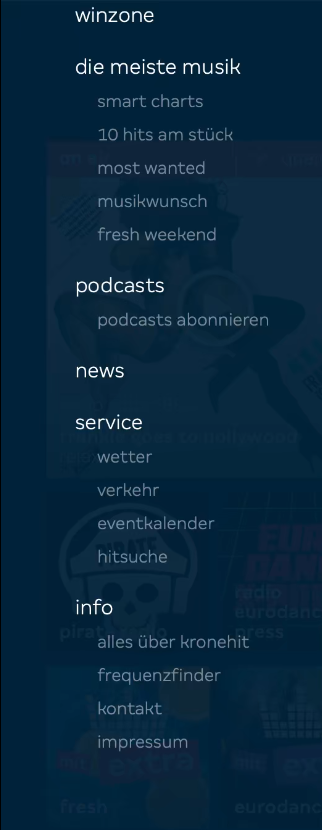
\includegraphics[scale=0.5]{Bilder/p03-ah-sidebar.png}
			\caption{Die Seitenleiste gibt eine sehr übersichtliche Zusammenfassung der Seiteninhalte}
		\end{center}
	\end{wrapfigure}
	Dass man den Radioplayer auf jeder Seite innerhalb von kronehit.at öffnen und neue Sender auswählen kann, wurde ebenfalls sehr positiv hervorgehoben\hyperref[sec:Anhang2]{$^2$}\label{ssub:radioplayer2}. \\
	\subsubsection{Seitenleiste}
	Ein weiteres nennenswertes Element ist die Seitenleiste. Von jeder Seite links oben erreichbar, gibt sie eine gute Zusammenfassung der angebotenen Funktionen, ist ästhetisch ansprechend und ohne Probleme benutzbar\hyperref[sec:Anhang3]{$^3$}\label{ssub:sidebar}.
	\clearpage
	\newpage
	\subsection{Negatives}
	\subsubsection{Tote Links und Standardfehlernachrichten}
	Als dringendstes Problem haben die Evaluierenden eine beunruhigende Menge an toten Links identifiziert. An mindestens zwei Stellen führen verlinkte Seiten zu einer nicht mehr existierenden Ressource. \\
	\begin{wrapfigure}{r}{0.4\textwidth}
		\begin{center}
			
\includegraphics[scale=0.296]{Bilder/notfound1.png}
			\caption{Eine Standardfehlernachricht in Alfred Hahns Moderatorenseite}
		\end{center}
	\end{wrapfigure}
	Ein solches Beispiel findet sich auf der Moderatorenseite von Alfred Hahn. Dabei erwähnt er sein neuestes Projekt: \enquote{kronehit late nite talks}. Ein Klick auf den hervorgehobenen Text führt jedoch zu einer Standard \enquote{Not Found} Seite\hyperref[sec:Anhang4]{$^3$}\label{ssub:notfound1}. Dieser Umstand ist aus zwei Perspektiven problematisch. \\

	Offensichtlicherweise sollten Links nicht ins Leere führen, jedoch sollte, falls es doch passiert, keine Standardfehlernachricht angezeigt werden, da das möglicherweise Informationen über die Hardware oder Software des Servers preisgibt. \\

	Auf der Moderatorenseite von Matthias Daniel gibt es einen weiteren toten Link, in der \enquote{BigCityBeats} verlinkt werden\hyperref[sec:Anhang5]{$^4$}\label{ssub:notfound2}. Hier erhält man jedoch eine an Kronehit angepasste Nachricht, dass diese Seite nicht gefunden worden sei, wodurch klar wird, dass eine solche zwar existiert, doch nicht immer verwendet wird.
	\paragraphlb{Verbesserungsvorschlag}
	Die beste Lösung wäre natürlich alle toten Links zu finden und zu eliminieren. Da dies jedoch nicht immer möglich ist, sollte zumindest sichergestellt werden, dass stets die eigene Fehlernachricht angezeigt wird, anstatt auf die Standardfehlernachricht der Website zurückzugreifen. Ein Weg um tote Links zeitnah zu finden, könnte auch sein, stets darüber informiert zu werden, wenn die \enquote{Nicht Gefunden} Seite aufgerufen wird, und von welcher Seite verlinkt wurde um diese schnell finden zu können.
	\subsubsection{KronehitTV auf iOS}
	Einige der als am scherwiegendsten erachteten Fehler traten nur in Safari für iOS auf, es kann jedoch angenommen werden, dass es sich um ein allgemeines Problem bei mobilen Endgeräten handelt. \\

	Zwei dieser Probleme geschehen bei Verwendung des Kronehit TV Players, welcher auf iOS ein vorgefertigtes Videolayout zu verwenden scheint. Dieses Layout stellt standardmäßig einen Knopf zum Einschalten von Untertiteln zur Verfügung. Kronehit TV hat jedoch keine Untertitel und auf der Desktopversion gibt es die Möglichkeit Unertitel einzustellen auch nicht. Es ist jedoch trotzdem möglich Closed Captioning Untertitel einzuschalten\hyperref[sec:Anhang6]{$^6$}\label{ssub:tvmobile1}.
	\newpage
	\begin{wrapfigure}[20]{l}{0.4\textwidth}
		\begin{center}
			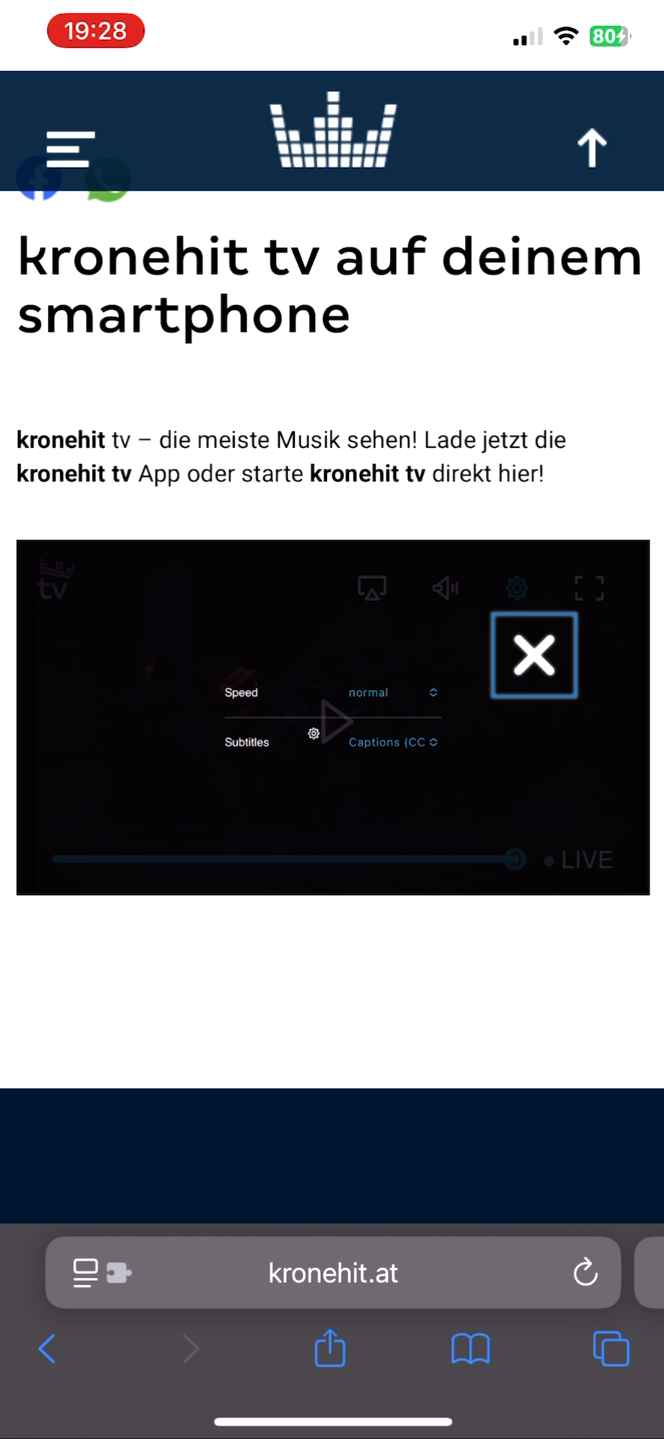
\includegraphics[scale=0.3]{Bilder/tvmobile.png}
			\caption{Player mit vergrößertem Knopf zum Schließen}
		\end{center}
	\end{wrapfigure}
	Ein weiteres, und bedeutend schwerwiegenderes Problem mit dem Player von KronehitTV sind die Einstellungen, welche innerhalb des Players verändert werden können, wenn es sich um eine Liveaufnahme handelt. Ein Klicken auf das Zahnrad öffnet ein Overlay über den gesamten Player und gibt erneut die Möglichkeit die Geschwindigkeit und Unertitel anzupassen. \\

	Obwohl jedoch in der rechten, oberen Ecke ein Kreuz zum vermeintlichen Schließen des Overlays existiert, führt ein Tippen darauf nur, dass es markiert und vergrößert wird. Um dieses Interface wieder schließen zu können, muss man die gesamte Seite neu laden\hyperref[sec:Anhang7]{$^7$}\label{ssub:tvmobile2}.
	\paragraphlb{Verbesserungsvorschlag}
	Beide der Player (Jeweils der für das Video und der Liveaufnahme) verwenden unterschiedliche Layouts, welche jedoch beide Funktionen anbieten die die Website gar nicht zur Verfügung stellt. Zur akuten Lösung des Problems wäre es eine gute Idee, das Layout der Player anzupassen damit keine Untertitel auswählbar sind. Zur Lösung der nicht schließbaren Einstellungen müsste man eventuell sogar den gesamten Knopf deaktivieren. \\
	\vfill
	\subsubsection{Doppelte Registrierung}
	Bei der Benutzererstellung wird nicht überprüft, ob eine E-Mail Adresse bereits im System registriert ist, oder nicht. Man kann die gleiche Adresse ein zweites Mal verwenden und das System verschickt sogar eine weitere Bestätigungsmail um seinen neuen Account zu bestätigen. Bei dieser zweiten Registrierung geschieht jedoch nichts, da man sich immer noch mit dem alten Passwort anmelden muss\hyperref[sec:Anhang8]{$^8$}\label{ssub:register}. Hierbei wäre es natürlich ein bedeutend größeres Problem, wenn man auf diese Weise ein Passwort ändern könnte. Wenn ein Benutzer sich jedoch fälschlicherweise einen zweiten Account erstellt, wird dieser in keinster Weise darüber informiert, dass bereits ein Account besteht, das gerade eingegebene Passwort nicht gültig sein wird oder stattdessen das Passwort besser mit der \enquote{Passwort vergessen?} Schaltfläche geändert werden sollte.
	\paragraphlb{Verbesserungsvorschlag}
	Vor Abschicken des Formulars, sollte in der Datenbank überprüft werden, ob ein Benutzer mit dieser E-Mail Adresse bereits existiert und eine Fehlermeldung ausgeben. Da der Prozess der Accounterstellung auf kronehit.at in mehrere Teile gespalten ist, könnte man schon bei der ersten Eingabe den Benutzer darüber informieren, dass er oder sie bereits einen Account hat.
	\newpage
	\subsubsection{Radioplayer}
	Der Radioplayer, welchen man nur aufrufen kann, wenn man im Footer auf dessen Link klickt, ignoriert oft, dass man gerade einen Sender zu seinen Favoriten hinzugefügt hat. Speziell das Herz auf der rechten unteren Seite scheint nie zu funktionieren. Interessanterweise erscheint, wenn man es verwendet, ein Popup, dass dieser Sender sich nun in den Favoriten befindet, was jedoch nicht stimmt. Es scheint, als ob man nur über die Sender in der linken Seitenleiste selbst erfolgreich einen Favoriten hinzufügen kann\hyperref[sec:Anhang9]{$^9$}\label{ssub:radio1}.
	\paragraphlb{Verbesserungsvorschlag}
	Da es sich um ein rein technisches Problem zu handeln scheint, wäre der beste Weg das Problem zu lösen, die Funktionsfähigkeit des Favoritenknopfes wiederherzustellen. Da der Knopf an allen anderen Orten standardgemäß zu funktionieren scheint, könnte es sein, dass die untere Leiste verändert wurde, und das zu dem Ausfall führte.
	\subsection{Analyse}
	Viele der schwerwiegendsten Fehler fallen in die Heuristiken der Fehlervermeidung und der umkehrbaren Aktionen. Einige der weniger dringlichen Probleme befassen sich auch mit der Konsistenz der Website. Daraus kann man schließen, dass viele der erkannten Probleme darauf zurückzuführen sind, dass Benutzer entweder nicht über ihre Aktionen oder die Aktionen des Systems informiert werden oder nicht in der Lage sind etwaige fehlerhafte Aktionen rückgängig zu machen. Während solche Probleme zu keinen fatalen Ergebnissen führen, können sie durchaus das Benutzererlebnis negativ beeinflussen. Besonders das Benutzererlebnis auf mobilen Endgeräten scheint oft zu leiden. Viele der erkannten Probleme geschehen höchstwahrscheinlich nur auf mobilen Browsern und auch wenn diese einzeln genommen keine hohe Bewertung erhalten haben, summieren sich diese doch und führen zu Frustration bei Endbenutzern. Jedoch muss auch erwähnt werden, dass das Erlebnis des Radiohörens auf der Website ein sehr gutes ist.
	\section{Fazit}
	Während die Grundfunktion der Website durchaus gegeben ist, fallen einem an vielen Orten technische Gebrechen und Designprobleme ins Auge. Eventuell wäre es ratsam sich auf spezifische Gebiete zu konzentrieren und diese Schrittweise anzupassen. Ein Beispiel wäre der dezidierte Radioplayer im Footer, da dieser in der Theorie eine sehr gute Idee ist, jedoch an vielen technischen Problemen leidet.
	\section{Quellen}
	Die Heuristiken welche in dieser Evaluation angewandt wurden, basieren auf \href{https://cdn.isds.tugraz.at/hci/reports/ss2017/g3-02-tugraz-en/heplan/heuristics.pdf}{Andrews Allgemeinen Usability Heuristiken} von Keith Andrews.
	\section{Anhang}
	\begin{itemize}
		\item[]{\label{sec:Anhang1}\hyperref[ssub:radioplayer1]{$\wedge$} 1) Siehe videos/p01\_SU\_MusikGehtWeiter.mov}
		\item[]{\label{sec:Anhang2}\hyperref[ssub:radioplayer2]{$\wedge$} 2) Siehe videos/p02\_SU\_KlickAufPfeil.mov}
		\item[]{\label{sec:Anhang3}\hyperref[ssub:sidebar]{$\wedge$} 3) Siehe images/p03\_ah\_sidebar.png}
		\item[]{\label{sec:Anhang4}\hyperref[ssub:notfound1]{$\wedge$} 4) Siehe videos/n01\_SU\_NotFoundError.mov}
		\item[]{\label{sec:Anhang5}\hyperref[ssub:notfound2]{$\wedge$} 5) Siehe videos/n01\_SU\_SeiteNichtGefunden.mov}
		\item[]{\label{sec:Anhang6}\hyperref[ssub:tvmobile1]{$\wedge$} 6) Siehe videos/n04\_SU\_UntertitelKronehitTV.MOV}
		\item[]{\label{sec:Anhang7}\hyperref[ssub:tvmobile2]{$\wedge$} 7) Siehe videos/n02\_SU\_KronehitTVNichtSchließen.mov}
		\item[]{\label{sec:Anhang8}\hyperref[ssub:register]{$\wedge$} 8) Siehe videos/n03\_ah\_double-register.mp4}
		\item[]{\label{sec:Anhang9}\hyperref[ssub:radio1]{$\wedge$} 9) Siehe videos/n05\_SU\_RadioplayerFavoriten.mov}
	\end{itemize}
























  
\end{document}